% =====================================================================
%  MSACL DS301 Deep Learning · Quiz 7 · Sequence Models and Attention
%  Academic problem-set style (single-source, \ifsolution toggle)
%  SINGLE SOURCE — produces BOTH the student quiz and the answer key.
%
%  ANSWER TOGGLE
%  -------------
%  Student version (answers HIDDEN) — the default:
%       pdflatex quiz05_attention.tex
%  Answer key (answers SHOWN):
%       pdflatex "\def\showsolutions{}\input{quiz05_attention.tex}"
%  (or, to flip by hand, change \solutionfalse to \solutiontrue below.)
% =====================================================================
\documentclass[11pt]{article}

\newif\ifsolution
\ifdefined\showsolutions \solutiontrue \else \solutionfalse \fi
% \solutiontrue   % <-- uncomment to hard-code the ANSWER KEY build

\usepackage[letterpaper, margin=0.6in, top=0.7in, bottom=0.5in]{geometry}
\usepackage{amsmath, amssymb}
\usepackage{xcolor}
\usepackage{tikz}
\usetikzlibrary{decorations.pathreplacing}
\usepackage{fancyhdr}

\pagestyle{fancy}
\fancyhf{}
\fancyhead[L]{\small\textbf{MSACL DS301 --- Deep Learning}}
\fancyhead[R]{\small\textbf{Quiz 7: Sequence Models and Attention\ifsolution\ \textmd{(Answer Key)}\fi}}
\fancyfoot[C]{\thepage}
\renewcommand{\headrulewidth}{0.4pt}

\newcommand{\blk}[1]{\underline{\hspace{#1}}}
% Reveal-or-blank: shows the answer in the key, a blank rule on the student sheet.
\newcommand{\rb}[2]{\ifsolution\textbf{#1}\else\blk{#2}\fi}
% Boxed answer (key only) and blank writing space (student only).
\newcommand{\keybox}[1]{\ifsolution\par\vspace{2pt}%
  \fbox{\parbox{0.965\textwidth}{\small\textbf{Answer.}\; #1}}\par\fi}
\newcommand{\work}[1]{\ifsolution\else\vspace{#1}\fi}

\setlength{\parindent}{0pt}
\setlength{\parskip}{3pt}
\setlength{\abovedisplayskip}{5pt}
\setlength{\belowdisplayskip}{5pt}

\begin{document}

\begin{center}
{\Large \textbf{Quiz 7 --- Sequence Models and Attention}}\\[2pt]
{\normalsize A mini attention heat map, one weighted average by hand, and the Q/K/V lookup}
\end{center}

\vspace{-2pt}
\begin{center}
\fbox{\parbox{0.92\textwidth}{\small
\textbf{Instructions:}\; Answer all three questions. Intuition first --- read the picture, then do
one small calculation. No calculators needed.%
\ifsolution\else\\[4pt]\textbf{Name:}\ \blk{6cm}\hfill\textbf{Date:}\ \blk{3.5cm}\fi
}}
\end{center}

\vspace{-2pt}\hrule\vspace{5pt}

% =========================== Q1 ===========================
\textbf{1. Read the attention heat map.}\; {\small A short peptide is tokenized one amino acid at a
time: \texttt{A -- C -- D -- E -- K}. The row below shows how much the last token, \textbf{K}
(lysine), attends to every token in the peptide --- darker = more attention. The five weights
already sum to 1.}

\vspace{6pt}
\begin{center}
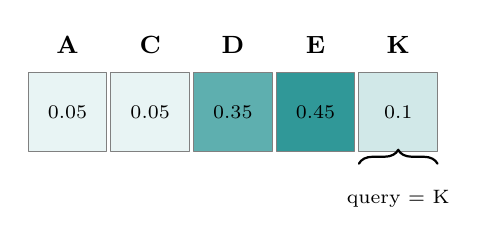
\begin{tikzpicture}[x=1.05cm, y=1.05cm, line cap=round, line join=round]
  \def\toks{A,C,D,E,K}
  \def\wts{0.05,0.05,0.35,0.45,0.10}
  \foreach \t [count=\i from 0] in \toks {
    \pgfmathsetmacro{\w}{ (\i==0)*0.05 + (\i==1)*0.05 + (\i==2)*0.35 + (\i==3)*0.45 + (\i==4)*0.10 }
    \pgfmathsetmacro{\op}{min(\w*1.8,0.92)}
    \fill[teal, opacity=\op] (\i,0) rectangle ++(0.95,0.95);
    \draw[gray] (\i,0) rectangle ++(0.95,0.95);
    \node at (\i+0.475,1.28) {\small\textbf{\t}};
    \node[font=\scriptsize] at (\i+0.475,0.475) {\w};
  }
  \draw[decorate,decoration={brace,amplitude=5pt},thick] (4,-0.15) -- (4.95,-0.15)
    node[midway,below=6pt,font=\scriptsize] {query = K};
\end{tikzpicture}
\end{center}

\vspace{4pt}
\textbf{(a)} Which token does \textbf{K} attend to \emph{most}?

\work{0.6cm}
\ifsolution\else\blk{4cm}\fi

\textbf{(b)} In one sentence, why might that be a \emph{chemically sensible} thing for the model to
have learned?

\work{1.0cm}
\ifsolution\else\blk{\linewidth}\fi

\keybox{(a) \textbf{E} (weight 0.45, the darkest cell) --- with D (0.35) a close second.
(b) \textbf{K is positively charged (basic)}, while \textbf{D and E are negatively charged
(acidic)} --- opposite charges attracting is exactly the kind of residue--residue relationship
(a salt bridge) a model trained on real sequences could plausibly pick up on, so K ``looking at''
the acidic residues nearby is a sensible pattern, not a random one.}

\vspace{2pt}\hrule\vspace{5pt}

% =========================== Q2 ===========================
\textbf{2. One weighted average, by hand.}\; {\small Attention's output is just a weighted average
of the token values, using the attention weights. Three tokens carry these (simplified to one
number each) values:}

\vspace{4pt}
\begin{center}
$v_1 = 4 \qquad v_2 = 10 \qquad v_3 = 1$
\end{center}

{\small The query's attention weights onto these three tokens (already summing to 1) are:}

\vspace{2pt}
\begin{center}
$w_1 = 0.5 \qquad w_2 = 0.3 \qquad w_3 = 0.2$
\end{center}

\vspace{4pt}
\textbf{Compute the attention output:}\; $\text{output} = w_1 v_1 + w_2 v_2 + w_3 v_3 = $

\work{1.2cm}
\ifsolution\else\blk{\linewidth}\fi

\keybox{$\text{output} = (0.5)(4) + (0.3)(10) + (0.2)(1) = 2 + 3 + 0.2 = \mathbf{5.2}$. Notice the
output leans toward $v_2=10$, the token with the biggest weight (0.3) --- that's all attention is:
blend the values, trusting the highly-weighted tokens more.}

\vspace{2pt}\hrule\vspace{5pt}

% =========================== Q3 ===========================
\textbf{3. Match the lookup roles.}\; {\small Self-attention is a soft lookup with three pieces per
token. Match each plain-language description to \textbf{Query}, \textbf{Key}, or \textbf{Value}
(each used once).}

\vspace{4pt}
\textbf{(a)} ``What I'm \emph{looking for}.''\hfill $\rightarrow$\;\rb{Query}{2.2cm}

\vspace{3pt}
\textbf{(b)} ``What I \emph{contain}, so others can decide if I'm relevant to them.''\hfill
$\rightarrow$\;\rb{Key}{2.2cm}

\vspace{3pt}
\textbf{(c)} ``What I actually \emph{give you} once you've decided I'm relevant.''\hfill
$\rightarrow$\;\rb{Value}{2.2cm}

\vspace{4pt}
\begin{center}
{\small \textbf{Word bank:}\;\; Query \;$\cdot$\; Key \;$\cdot$\; Value}
\end{center}

\keybox{(a) \textbf{Query} --- the question a token is asking. (b) \textbf{Key} --- the advertisement
a token puts out about itself, matched against every query. (c) \textbf{Value} --- the actual content
handed over once a query--key match says ``pay attention to me.'' \emph{The heat map in Q1 is
exactly Query(K) matched against every token's Key; Q2's weighted average is exactly the Value
mixing step.}}

\vspace{4pt}\hrule\vspace{3pt}
{\small\itshape \ifsolution Answer key.\else Keep this sheet --- Lecture 8 builds the full
transformer directly on top of this Q/K/V lookup.\fi}

\end{document}
